\documentclass[crop, tikz]{standalone}
\usepackage{tikz}
\usepackage{pgfplots}

\begin{document}
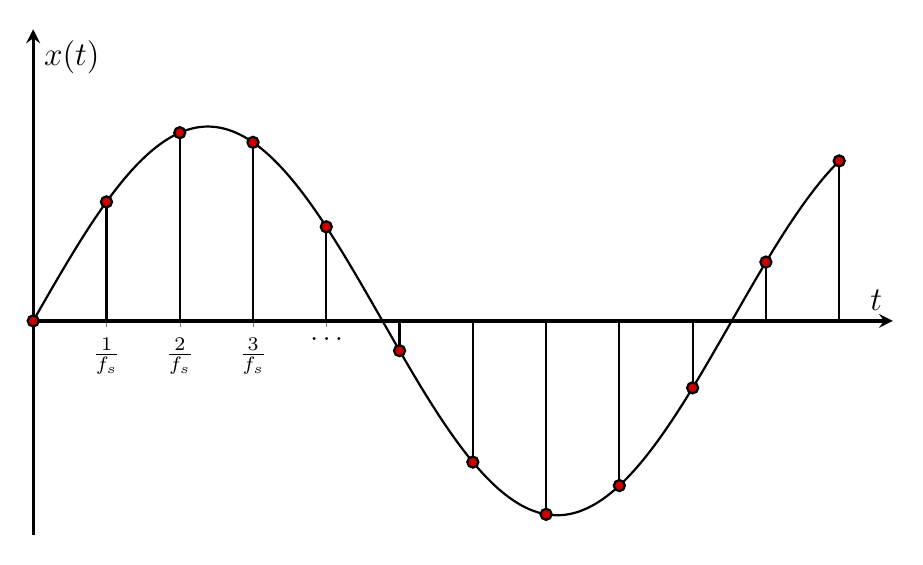
\begin{tikzpicture}
	\begin{axis}[
		width=12.5cm, height=8cm,
		xtick=\empty,
		ytick=\empty,
		xlabel={\large $t$},
		ylabel={\large $x(t)$},
		xmin=0, xmax=16,
		ymin=-1.1, ymax=1.5,
		xtick={1.365,  2.73, 4.095, 5.46},
		xticklabels={$\frac{1}{f_s}$, $\frac{2}{f_s}$, $\frac{3}{f_s}$, $\dots$},
		axis lines = middle,
		very thick,
		domain = 0:15
	]
		\addplot[no markers, samples = 100, smooth ,thick] {sin(2*180*x/13)};
		\addplot+[ycomb, mark=*, mark color=blue, samples= 12, black, thick] {sin(2*180*x/13)};
	\end{axis}
\end{tikzpicture}
\end{document}
